% Author: Izaak Neutelings (October 2020)
% Inspiration: https://tex.stackexchange.com/questions/25531/adding-underbrace-in-tikz
\documentclass[border=3pt,tikz]{standalone}
\usepackage{physics}
\usepackage{tikz}
\usetikzlibrary{calc}
\usetikzlibrary{angles,quotes} % for pic
\tikzset{>=latex} % for LaTeX arrow head

\colorlet{xcol}{blue!70!black}
\colorlet{vcol}{green!60!black}
\colorlet{myred}{red!65!black}
\colorlet{mypurple}{blue!60!red!80}
\colorlet{acol}{red!50!blue!80!black!80}
\tikzstyle{CM}=[red!40!black,fill=red!80!black!80]
\tikzstyle{rvec}=[->,xcol,very thick,line cap=round]
\tikzstyle{force}=[->,myred,very thick,line cap=round]
\tikzstyle{mass}=[line width=0.6,red!30!black,fill=red!40!black!10,rounded corners=1,
                  top color=red!40!black!20,bottom color=red!40!black!10,shading angle=20]
\tikzstyle{rope}=[brown!30!black,fill=brown!70!black,line width=0.4]
\tikzstyle{limb}=[thick,line cap=round]

\tikzset{
  pics/Tin/.style={
    code={
      \def\R{0.12}
      \draw[pic actions,line width=0.6,#1,fill=white] % ,thick
        (0,0) circle (\R) (-135:.75*\R) -- (45:.75*\R) (-45:.75*\R) -- (135:.75*\R);
  }},
  pics/Tout/.style={
    code={
      \def\R{0.12}
      \draw[pic actions,line width=0.6,#1,fill=white] (0,0) circle (\R);
      \fill[pic actions,#1] (0,0) circle (0.3*\R);
  }},
  pics/Tin/.default=mypurple,
  pics/Tout/.default=mypurple,
}

\begin{document}


% TIGHT ROPE arms
\def\L{3.2}   % length
\def\T{0.08}  % plank thickness
\def\H{2.2}   % human height
\def\CM{0.06} % CM radius


% TIGHT ROPE - weights - forces
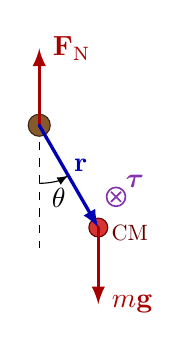
\begin{tikzpicture}
    \def\R{1.5}
    \def\F{0.65*\R}
    \def\ang{30}
    \coordinate (O) at (0,0);
    \coordinate (B) at (0,{-1.2*\R*cos(\ang)});
    \coordinate (CM) at (-90+\ang:\R);
    \coordinate (T) at ($(CM)+(60:0.3*\R)$);
    \draw[dashed] (O) -- (B);
    \draw[rope] (O) circle (0.14);
    \draw[CM] (CM) circle(0.12) node[below=2,right=2,scale=0.8] {CM};
    \draw[force] (O) --++ (0,\F) node[right=1] {$\vb{F}_\mathrm{N}$};
    \draw[force] (CM) --++ (0,-\F) node[right=1] {$m\vb{g}$};
    \pic[scale=1] at (T) {Tin};
    \node[mypurple,above right=0] at (T) {$\vb*\tau$};
    \draw[rvec] (O) -- (CM) node[midway,above right=-2] {$\vb{r}$};
    \draw pic[->,"$\theta$",draw,angle radius=21,angle eccentricity=1.3] {angle=B--O--CM};
\end{tikzpicture}


\end{document}